\chapter{The World of Haeckel}\label{world}
\pagecolor{gray}\afterpage{\nopagecolor}

%\begin{centering}
% \includegraphics{...}
%\end{centering}

\newpage

\pagecolor{gray}\afterpage{\nopagecolor}
\fontfamily{pzc}
\selectfont
Co-Consul of Ablon enters the Office and the General Autorius sits at his table, golden goblets of wine and a plate full of grapes rests easy in front of him. 

``We had an agreement, that we'd share all revenue.''

``Yes''

``Hereopolis has agreed to give you 20,000 pounds of gold. I want my share.''

``Who told you this?''

``You deny?''

``Who told him.''

``I have spies among his people.''

``If Herod is kind enough to give me a gift, what business is it of yours? A gift is not revenue.''

It is not a gift, it is a bribe. For political and military favours. The cost of which favours shall be born by the state.''

``Peasantry.''

``Let us be realistic. This arrangement of ours can not work if you seek every opportunity to aggrandize yourself at my expense.''

``Laughter. Aggrandize myself. This from the boy whose so called father has been declared a God.''

``An honour he well deserves.''

``You only did it so you might be known as the Son of a God. You have no accomplishments of your own, so you seek to borrow the glory of others.''

``Its true, it was no accomplishment to defeat you at Mutina.''

``You defeated me? You cowardly little shit. You never left your tent. You have never defeated me, in anything.''

``Gentlemen, lets not get overheated. Im sure we can come to some reasonable agreement. I had hoped that you had learnt some humility and discipline. You are still the same old crude, arrogant, lech that you always were.''

``Thats right. Just the same. The same that is still fucking your mother!''
\normalfont

\newpage
\begin{multicols}{2}

Haeckel is a land caught in a perpetual conflict between the common man's reality and the unspeakable horrors of the unknown. It is a home to foul horrors and nightmares made manifest. It's rulers are in constant fear of history relapsing, many feel the doors that lead to the Great War will open once again, spilling atrocities and nightmarish creatures stalking every countryside. To the common people this history is nothing more than an old wives tale meant to keep children in check. Other houses seek to manipulate the knowledge of history to suit their own ambitions. Here deceit is king, whether it be a supernatural horror disguising itself as a beautiful countryside, or the princely noble offering salvation but to a price worth remaining in damnation, or the lowly commoner that is fed lies all his life \ldots

\subsection{How to use this book}
This book provides you everything you need to know to play in the world of Haeckel. Anything that the players should not know immediately will not be described in this book. Each character will not know everything in this book; that is for the player to responsibly decide what he knows.

\begin{framed}\centering
We have chosen to include design commentary as part of this book so that Players and GMs can feast on it and satisfy their curiousity. Anything in this framed box will be that. This is intended to help people get an idea of what to expect in games in Haeckel or for them to enrich their own campaigns.
\end{framed}
%\begin{framed}\centering
% a pantheon of recurring "pseudomythological" entities and a collection of arcane books that supposedly yield insights into the mythology
% \end{framed}
\subsection{Chapter by Chapter} 

\section{Genre}

Haeckel is a vast world. The seven provinces of the old empire together are as large as Western Europe. The vast expanses of North Wall as big as alaska, or maybe even doubly so. It is this size that means that Haeckel defies exact definition. Painted in broad strokes it is possible to make some overall conclusions on its genre. 

Like most RPG settings it can be described as dark fantasy. It has drawn significant influence from literature and media such as REH's Conan, and could even be described as pulp fantasy. But that doesnt really help. For instance, Midgaard is a Kingdom carved in two by political intrigue. Part of it is influenced by Arthurian legend, but with a Gothic Horror type spin that takes it in a new direction. 

In stark contrast, the Megacity State of Ablon draw from the glorious golden age of Rome. Brouliard draws from the Golden Age of the French Chivalric Enlightenment. Culturally its in the renaissance - and often neglected cultural level - and has reached the age of gunpowder.  

Overall it would be fair to say that Haeckel is a milkshake of dark fantasy, pulp fiction, gothic horror with an emphasis on atmosphere, and historical fiction.

\section{The Realm of Haeckel}

\subsection{The Dread Gates} Deep within the impassible mountain range known as North Wall lies the Gate of Ignis, lord of the Flame. When Aratron and Ma’asei imprisoned the other Gods, it is said that Ignis was spared and that his flame was necessary to restore the balance and that another creature, one powerful enough to take to challenge the fire god was imprisoned. Haunting howls and strange lights are reported to emanate in the further reaches of North Wall. Many have attributed these phenomenons to the Gate of Ignis. No one who has ever found it has ever returned, to tell their story.

North Wall is a frontier zone, filled with miners hoping find fortune in the mineral rich mountains, pioneers looking to build a new life, adventurers searching for a rumored lost Kingdom beyond the mountains and those who are looking to hide. North Wall also has its own native secrets hidden within the mountains, giants whom are said to be the children of Ignis, creatures who prey on children who stray too far from their parents, snow like wolves that seem to stalk hunters from unreachable areas, living gems waiting for unfortunate minors to step into their clutches.

In the world of Haeckel there are a total of Seven such Dread Gates. Finding and unlocking their powers are the subject of entire campaigns. Secret Societies in Haeckel are constantly trying to find them and the nature of the Dread Gate's boons is incredibly esoteric. It is said that to unlock them require great sacrifice in the form of a Ritual.

\begin{figure}[h]
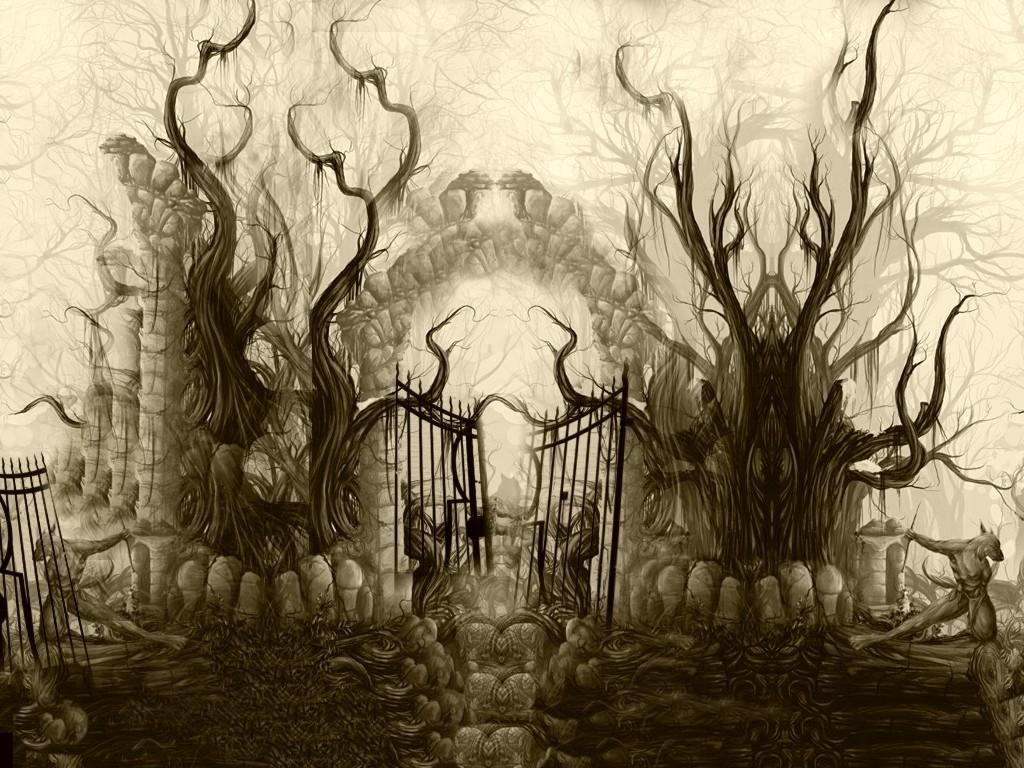
\includegraphics[width=\columnwidth]{gates-of-hell-open}
\end{figure}

\subsection{The Powers That Be} Power exists where people believe it exists. It is both fickle, complex, and its ramifications are terrifying. The World of Haeckel has both overt and covert powers that shape its very existence; past, present, and future. 

\subsection{The Invisible War} Since Antiquity the Mages of Haeckel have been in perpetual war with each other from behind the scenes. The 1000 years of bloodshed have stained the land. The Nobles and Powers That Be whom dominate the world have ensured that the details of this conflict remain in secret. To the common man the Invisible War is a shadowy myth that is best ignored. The reality of this War is simple. In Haeckel, the cost of developing arcane research is immense. In a bygone era, some Mages sought to channel the wealth of nations in order to fund it. They are an extremely secretive lot and they often use advanced techniques to ensure that no other Mage can acquire their secrets. In financial terms, the cheapest way for a Mage to gain new power is for him to slay another Mage and steal their knowledge. Thus, every Mage is compelled by the nature of their work to hide in the shadows and avoid drawing attention to themselves lest they be preyed upon by other more dangerous individuals. This however has some extra complexity. You see, the most powerful mages are not interested in the small fish mages. They want them to grow in power, so that one day they may take their work for themselves. At the same time, some Mages realise that very complex tactics has evolved from this conflict. Weaker mages are often used as bait by more powerful Mages in order to ambush other powerful predator Mages. Thus you have this complex game of cat and mouse. 

\paragraph{The esoteric nature of Magic} In most Player's Handbook type products there exists a sizable chapter on spells that exist within the game. We have chosen to explicitely omit this from here. In Haeckel RPG magic spells are a source of mystery, wonder, and an integral part of the joys of discovery for players. Simply put, it is an overt declaration that the players will not know what to expect with regards to magic. That is fundamental to its esoteric nature. Even the way that magic works is unknown initially. There are a number of Magical Theories, some work, and some dont - and puzzilingly some that work might even contradict each other working systems. 


\section{History}

\begin{tabular}{l|r}
    \hline
    Year & Event \\
    \hline
    0    & The First Apocalypse \\
    350 & The Invisible War Begins \\
    950 & The Time of Summer \\
    1250 & The Great Catastrophe \\
    1251 & The Great War \\
    xxx & The Hour of the Knife \\
    1350 & Current Day \\
\end{tabular}


The study of Haeckel's past can prove to be a maddening exercise. The denizens of Haeckel have rich cultures and histories dating back centuries. Some of it is mythical and some of it grounded in fact - albeit interpreted by the Powers That Be to suit their own needs. Through a long tradition, and a shared history, the provinces of Haeckel have adopted the Haeckelian calendar to mark the passing of years. Isolated areas however may track time through their own reckoning. 

\subsection{The Time Before}

The true origins of Haeckel remain a mystery. Gypsy,  Elven, and Dwarven legends, as well as numerous creation myths suggest that the current inhabitants are descendents of a terrible race from a Land Beyond whom migrated to Haeckel. Though at times contradictory, common themes hint that the continent may have existed for eons, forever ebbing and flowing in an eternal cycle of expansion and decay. 

\subsection{The Long Summer} 

\subsection{The Fall} Janus Thurinus blessed King of Haeckel, unifier of Seven Territories, Keeper of Justice and Bridge between the Elven and Man. Under his rule Haeckel thrived in an era of peace and prosperity. This era is also known as the Time of Summer, for The Fall that was to proceed.
In the final years of Janus Thurinus' reign, incompetent eunuchs deceived the queen and persecute good officials, and the government becomes extremely corrupt on all levels. The elites of society allowed degradation to occur, using the political chaos as a shroud to mask their illegal occult practices. A rebellion breaks out lead by the perpetrator of the chaos Wiglaf Lysander, High Constable of Haeckel’s Royal Guard. The rebellion is barely suppressed by the troops under the command of Gestae Ni, Vice Captain of the Royal Guards. Meanwhile Imperial Wizard and Queen's Advisor, Luoyang Xi, attempts to halt a growing cult within the ruling nobels known as The Phex. Louyang uncovers a plot to open up a legendary Dread Gate, ignored by the Queen who is fighting to save her kingdom and repair harm caused by the rebellion, Louyang Xi decides to confront the cult. He interrupts their ritual causing a catastrophic chain of events leading to the destruction of the capital, ultimately shattering the Kingdom of Haeckel and cursing its land. This event has been dubbed the Great Catastrophe. A great quake splitting a region of Brouilard in two, opening a great chasm known as The Scar of Rock Rose, weather takes a more magical property causing strange toxic storms which scorch the land, strange plagues that seem to have an intelligence of their own mutating its victims. Horrors that were once fables made manifest stalk the realm. Haeckel’s days of Summer now a fading memory.

Though devastated and torn the rebellion continues and many of its culprits survive The Great Catastrophe. After the dust settles the young Prince Aglar is found by soldiers of Wiglaf Lysander, who proceeds to seize control of the imperial capital under the pretext of protecting the Prince. Wiglaf Lysander also initiates a murderous campaign to recover Imperial relics lost due to Great Catastrophe. Imperial chancellor Ozymandius escapes and issues an imperial edict in the Queen's name to all regional warlords and governors, calling them to rise up against Wiglaf. Under Gestae Ni's leadership, [[[wiki:the-eighteen-warlords | eighteen warlords and mercenary companies form a coalition force in a campaign against Wiglaf, but undermined by poor leadership and conflict of interest, they only manage to drive Wiglaf from the capital to the ruins of Midgaard. Wiglaf is eventually killed by a mercenary in dispute over a lost Royal Relic. Alisuim of Yares, healer and matriarch to a militia of medics and priests finds the Imperial Seal and keeps it secretly for herself, further weakening royal authority. Without a strong central government, warlords begin to rise and fight each other for land, plunging Haeckel into a state of anarchy. Mysteriously once dissolved noble House, Mordenheim, has rekindled and has reported to be lead by Wiglaf's assassin, the former mercenary captain; now, Dracs von Mordenheim. Dracs von Mordenheim then established the mysterious Order of the Grim Shadow and rallied a small army to battle his former employer Ba'al Xebub, sovereign Merchant King of Abyssal. Remnants of the Lysander family have waged a blood feud against the Mordenheims.

\subsection{The Great War} The Great War spanned a generation. The Great War was one of attrition, such the magnitude that most of Haeckel may never recover from. Lands stripped of resources to produce terrifying war machines, towns and villages depopulated forcing all able bodied person to fight for either side. Lysander’s blood feud depleting the Wiglaf family tree, forcing The Dark to make unholy pacts with the dark coven of The Phex. Soldiers fleeing from encounters with The Dark report seeing their generals transforming into horrifying unkillable man-beasts. The forces of Ba’al Xebub also suffered heavy losses, with income depleted Ba’al forced to sell of his treasury piece by piece to fund his vast mercenary army. Rumors amongst Abyssimiar and Ubris Furor tell the story of Minotaurs visiting towns, villages and desert camps to force the populace in to slave armies. The Order of The Grim Shadow too suffered heavy losses, perhaps the heaviest being their leader’s loss of humanity. The once loved leader became more and more reclusive. Rumors throughout western Haeckel tell tales of House Mordenheim experimenting in the forbidden art of Necromancy to create an army that could never deplete. Other and perhaps more troubling reports tell of the members of House Mordenheim being monsters who Bleed of Shadows.

Unbeknownst to The Dark, Prince Aglar was spirited away at the start of the Great War by Alisuim. Protected and groomed to bring forth a new era of peace and reunify Haeckel, Prince Aglar rallies the remaining allies to the fallen throne and enters the melee as The Principality of Thurinus. With the combined might of those whom view the Principality with an almost religious zealous they emerge victorious battle after battle, even halting the march of The Order of The Grim Shadow’s undead army.

The juggernaut that was The Great War is slowly coming to a halt. Due to successful sabotage attempts to all other factions The Principality’s goals are well within reach. Ba’al Xebub’s forces now feeble and non existant, many mercenary companies revert into banditry, Minotaurs abandoning their former master on a quest to reestablish their ancient homelands. The family of the Dark, despite having bestowed unholy blessings becomes almost extinct. The power over the undead horde ebbs and fades leaving only the members of House Mordenheim as The Order’s military might.
Yet despite The Principality’s military quickly regaining control of Haeckel, Dracs still pushes on his quest for revenge. With only four members of House Mordenheim, The Order of the Grim Shadow manages to slaughter all but one member of Wiglaf’s lineage; leaving the sole survivor to lament over his families short comings. He then encounters Prince Aglar with his closest ally House Liebentod within Ba’al’s Obsidian Spire within Abyssimiar. A battle ensues, and none seemed the victor. Despite the strange and perhaps unholy nature of the members of House Mordenheim they could not slay these zealots. Recognizing the passion within his opposition to that of his own Dracs surrendered, only on the condition that he alone may finish his ascend to the top of the spire so that he may meet Ba’al face to face.

Before facing Ba’al, Dracs faced his former general comrades, all whom too weary to continue the war. Nothing is known of the meeting between the two, only that Dracs descended the tower and that no one has ever sighted Ba’al again. From the meeting between the two forces, House Liebentod defected from the Principality to join that of The Order of The Grim Shadow. This caused a brief tension between the two remaining forces and caused rifts to open within the Principality, some members rallying for the destruction of the Order, while others expect House Liebentod to pacify The Order of The Grim Shadow. Within a week Dracs himself met with the Prince and swore fealty to the throne and assisted Prince Aglar using The Order of The Grim Shadow to aid his quest in unification. Prince Aglar in turn recognized House Mordenheim as a legitimate noble house of the highest regard. Despite bringing a degree peace to Haeckel this action formed a permanent divide within the Principality. Those who remained distrustful of House Mordenheim, distant themselves from the Prince, silently plotting the demise of House Mordenheim, some even plotting the demise of Prince Aglar.

\subsection{The Hour of the Knife} The Great War had officially ended, and although The Principality of Thurinus had won the war, their ultimate goal of peace and unification was lost. Noble houses became more and more distrustful of one another, the leaders of several houses turn missing or have been reported to have been assassinated. Veterans of the war roamed the land scavenging a looting all that they can. Once enslaved creatures used to terrorize enemies now left unchecked and prey upon helpless villagers. The Great Houses of Ablon who stayed neutral during the Great War, since then Ablon has become increasingly distant instituting an isolationist policy. Due to the magical horrors that were unleashed upon the world a number of veterans from all factions have banded together to form an organization, calling themselves The Puritans; these men and women have vowed to cleanse Haeckel of all magic. A group of mercenaries have found new methods to survive during a time of peace, now hiring themselves to that of common man as a means to enforce justice; The Company is called The Enkertons. The survivors of The Dark, left torn and broken have found ways to survive Ignis, the sole survivor of the Wiglaf lineage, slowly rebuilds his family. As new factions form many old ones meet violent ends. A string of assassinations stretch over Haeckel, the mysterious group known as The Phex becomes more active as knowledge of The Dread Gates scattered across the land slowly become more available to those who seek them.

Dracs von Mordenheim is reported have met his demise on the end of an assassin’s blade, the suspected culprit a sleeper agent of The Phex. Shortly after the death of Dracs, his sworn ally the Prince Aglar disappears, his fate unknown. He leaves the Principality with twin sons whom grow up to hold different views on how Haeckel should be protected. In the wake of the war a total of 24 Houses suffered mysterious fates, some never recovering after the death of their liege lord. It is unknown whether all of these deaths and disappearances are due to some Phexian plot.

\subsection{The Present} 

\section{The Geography of Haeckel}

Depending on ones outlook the inhabitents of Haeckel call it by different names. Like the chest of a sleeping beast the world of Haeckel expands and contracts according to the needs of the Dictators whom rule it. Cartography, the art of mapping, is a lost art. Some live a claustrophobic existence; living and dieing for their entire lives within 20 miles from their place of birth. Some others with more intimate understandings of the land greedily hoard these secrets for it is a key advantage to attaining wealth. 

Untold millions of Humans exist in Haeckel. Their lives are brief, flickering lights, trapped in drudging poverty as farmers whom cultivate the land. Hundreds of small cities dot the land. Towns and villages are innumerable, to map it would be futile. While this may seem really dense, the reality is that only cities are a dense mass of bodies all compressed together like sardines in a small area. Haeckel mirrors Western Europe in geographical area and is actually quite depopulated. Land, and thus grain output, is the ultimate measure of wealth for any landed nobility; though, multiple schools of thought exist on the nature of power in Haeckel.

Haeckel can be thought of as having Seven Kingdoms, each with a united history that loosely ties it together as they lived together before the Fall under the vast shadow of the Empire with its center in Avalonia. To the north of the old Imperial states is North Wall. It is the howling abyss of the world, a land of unimaginable size with a breadth that cannot be measured. To the south is the independent Kingdom of Abyssimiar. To the native Haeckelians, Abyssimiar is an exotic realm that is both eerie and terrifying due to its alien culture. Abyssimiar managed to stay independent by virtue of its powerful navy and extremely harsh deserts that contributed to its geo-political isolation. Even further south is the Southern Continent, the realm of the Unknown. It is virtually cut off from the rest of Haeckel but its creeping influence grows year by year like worms in shit.

\begin{framed}\centering
Part of the appeal of exploratory game design is learning the world and getting map awareness is a key part of the game. Going from a scared little guy with no idea whats in the world to a hardened adventurer able to navigate his way through the entire world with little sweat. 

To this end, significant thought has been put into promoting exploration in the game mechanics. This is both exploration in the sense that you travel around and in the sense that you be creative with the in-game content. For example, the Alchemy and Herbalism systems promote exploration since you must find ingredients and experiment with them to see what happens. It is one of the design mantras that we have aspired to.
\end{framed}

% Petty jealousies give birth to considerable envy.  
% Law of the Minimum
% A Legend, a Prophecy, that their Leader will come from a foreign land and guide them to true Freedom. The people here are simple and survive on hope. 

% Government claims are not tantamount to the truth


\definecolor{shadecolor}{gray}{0.9}
%\begin{shaded} text \end{shaded}

\begin{snugshade} "I live solely for myself, and there is no end to it, as long as there are people to kill in this world I will never disappear." -- Ordrelan \end{snugshade}


% Maxims of Madness
% Tenets of Terror
% Doctrines of Damnation
% Creed of ...
% Fundamentals of Fear
\paragraph{Exploration \& Campaign Play} 

%   
 
% Exploration is promoted
% Non-linear gameplay.
% Complete the dungeons in any order that you want.
% The game is full of secrets that promote exploration. There is no artificial limits stopping you from doing certain things. If you get something, you can play with it. 
% Learning the world and getting map awareness is a key part of the game.
% Take any road you want. Bends over backwards to reward and reinforce exploration. The only way to learn about the world is to explore. You may end up wandering the world and getting your butt handed to you, but thats fine. 
% It minimises the risk of dieing and frustration from it by speeding up the character creation system so you can rapidly get back into the game. If you die, and lose some loot, you could try find it again with a new character.
% Its upto the players to find landmarks and make note of them.
% Go from a scared little guy with no idea whats in the world to a a hardened adventurer able to navigate his way through the entire world with little sweat. 

% Choosing paying taxes or not
% Items
% No challenge system to balance encounters against the players. Its upto the players to decide if they're capable enough to deal with a situation
% Learning how capable you are is part of the exploration of the game
% 
% % Brazier
% % Potted Plant
% % Fountain

\paragraph{Political Intrigue} The Kingdoms of the Old Empire compete viciously on the nation state stage. And within those Kingdoms cutt throat politics and scandal is rife as the various power players thirst for an even greater slice of the pie. Political intrigue is one of the most common overrarching themes to the narrative in Haeckelian campaigns. Also, a significant proportion of the system is built so that the players may immerse themselves in it.

\begin{snugshade} "And so it begins. The trap is set. Centuries of humiliation visited upon my family will be avenged. Their plan is elegant and vicious. At the moment of his greatest confidence, traitor strikes. Pervading common wisdom is the mark of every great conspiracy. Even though they would never admit it, a popular man always has many who want to get rid of him. Our House will be more powerful than ever. Alone and vulnerable at the edge of society, we will make them come face to face with fear. We will make them turn on each other like rats in a flood." -- Raakarth \end{snugshade}

\paragraph{Discovery and Exploration} A key component of Haeckel that distinguishes it from other RPG settings is the concept that the vast majority of the content needs to be discovered in the game and thus are GM secrets. There will be an entire Herbalism and Alchemy subsystems, for example, built for such a purpose among many other things. 

Therefore the purpose of this book is to help the players build characters that fit within the setting and are provided enough ammunition to build powerfully evocative characters that they could then breath life into in new and interesting ways. 

\paragraph{Character Gameplay} We aimed to promote ways such that different character types have a genuinely different gameplay feel. There would be different routes through the gameplay world, in which different obstacles are faced, and different tactical options for various situations. This idea has influenced our module design where we promote replayability. 
 
\paragraph{Craftsmanship} 


%\subsection{Themes}
%
%When we set about creating a setting with some roots in pulp fiction we immediately thought of Lovecraft and the repeating themes used in his works. Typically they would revolve around ignorance vs knowledge and the standard norms of society being shaken by something foreign. Dracs' imagination drifted towards more modern medias. Italian exploitation horror (grind-house films, as some have dubbed) - which I would consider to be the modern film equivalent to pulp fantasy fiction and 80's horror films. 
%
%\paragraph{Ignorance vs Knowledge}
%\paragraph{Pandora's Box}
%
%\subsection{Current History}
%Roughly one hundred years ago a supernatural apocalypse and brutal civil war occurred that rocked the continent. The Old Empire had fallen, and each of the seven provinces of the Empire now act as independent states. A number of other regions existed as independent states outside of the Empire. The tragedies and bitter conflicts of the past still scar the land. History has not been forgotten and sets the tone for the present. 
%
%The seven ex-imperial provinces are: Ablon, Avalonia, Brouliard, Midgaard, Nes, Nosquam and Ubris Furor. 
%
%The foreign provinces are: Abyssimiar, North Wall, Grul, and the Southern Continent.

%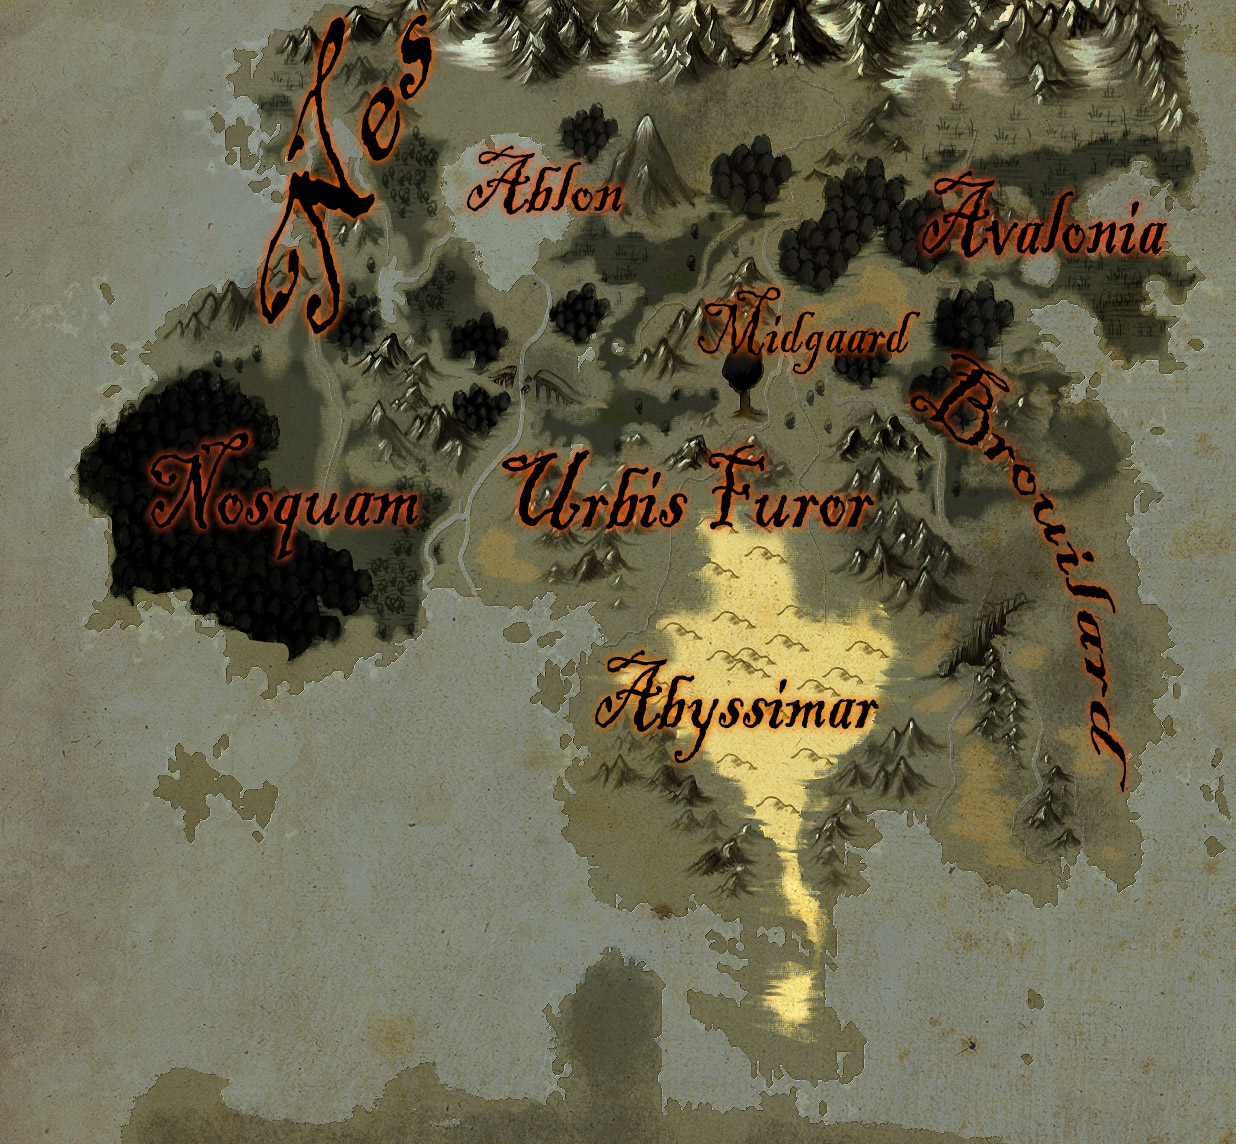
\includegraphics[height=\textheight, width=\textwidth]{Haeckelmap.jpg}
        
%\ThisCenterWallPaper{1}{Haeckelmap.jpg}

\subsection{Ablon} 

The incomprehensibly vast Mega City of Ablon casts a tremendous shadow over the world. Its influence is far-reaching and its achievements are prodigious and monumental. Three great Houses rule Ablon with ironfists, their powers are sweeping and their desire to see each other's downfall is boundless. Tales of their ambitions are widely known and it is said that they seek to make the Mega City State into an Empire in its own right. Many other smaller cities exist within the greedy aegis of Ablon, all are puppets that's sole purpose is to provide grain to the capital of this region. The decadence, wealth, and architecture of Ablon is lofty and unforgettable as it sets the standard for all of Humanity.  

Naming Scheme: Roman and Greek

\subsection{Avalonia} 

The Old Capital. Wasteland of the Old Empire and the most valuable province in the known world. Because it is here and only here where magic is found in its most raw form. Without the phex, there would be no Powers That Be. The greatest treasure in the known world. It is here where the only opened Dread Gate exists. The Mages that control it control the destiny of the Old Empire. But despite this, it is locked in a never ending struggle to survive against supernatural horrors. Those few survivors that stubbornly remain do so at a terrible cost as they must survive without the protection of civilisation in a stone age existence.

Naming Scheme: Arthurian and Latin

Avalonia is a province that is drenched in horrific myth and legend. Vast amounts of misinformation exists outside of this land. Mundane characters would likewise be trapped in this maelstrom of misinformation. Avalonia is a land where the unreality is breaching reality. Only Mages would have even a modicum of understanding about the true natures of this realm. 
\begin{figure}[h]
\includegraphics[width=\columnwidth]{avalonia4}
\end{figure}

%\begin{multicols}{2}
\subsection{Brouliard} 

Filled with every kind of social insect, Brouliard is a grand masquerade teetering on disaster. The cities have embraced the ideals of the Enlightenment and reached a Golden Age of Prosperity under the absolute rule of Queen Sophia. Brouliard is now the cultural diamond of the known world but it still wrestles endlessly with its barbaric past.

Brouliard society is a tangled web of competing forces. Brouliard civilisation rests on a political tripod; the most unstable of structures. A deceptive balance of power exists between the Absolute Queen Sophia, the Other Society and powerful Merchant Houses. It is complicated by a feudal trading culture and a political past of absolute tyranny. 

Naming Scheme: French, Greek, and Early Germanic

% width=0.5\textwidth, height=0.5\textheight

%\end{multicols}
% The cultural diamond of Haeckel. Queen Sophia has produced a Golden Age of prosperity for her people. This land is based of Renaissance and Chivalric France as well as 18th century Russia. Its a land that is progressing towards the Enlightenment but paradoxically the benevolent ruler Queen Sophia is also an Absolute Monarch and a Tyrant. 

% Be sure he recalls his flimsy denials before the face of death's sweet smile. 

% Better to miss an opportunity than invite disaster
% My people are cautious and pragmatic.


\subsection{Midgaard} 

Midgaard is a realm both glorious and terrible. It is a grand tapestry of gothic medieval horror. Within this blood drenched kingdom, life is countlessly born, and unceasingly ended in almost cyclical conflict. The Lords of this land are doomed souls tarnished forever by the sins of ambition, pride, honour, and glory. The battle against evil can be daunting - even terrifying - but not futile. Most stew hopelessly, drunk on their desires, but those special few are martyrs who end up choosing death over damnation.

The people of Midgaard are fearful, fanatical, and violent lot. Alone, peasants are weak and cowardly. But as a mob they can quickly become vicious like a bloodthirsty pack of wolves. The chorus of baying peasants as they burn a witch is to be seen. Civilisation is not safe as it once was; savage bands of bandits roam the countryside that attack, murder, and pillage unprovoked, using speed and shock tactics to stay alive.

In Midgaard, the unnatural is accentuated by emphasising the natural. For every prowling night terror, remember the village of decent folk it preys upon. For every tale of obsession and betrayal, consider the families whose loving ties see them through the years. In this Kingdom there is a distinct contrast between wondrous and wrong.

Naming Scheme: Arthurian, Middle English, Babylonian

% The land of Gothic Horror, Medieval Fantasy, and Arthurian legends. This land has an English and French medieval theme that aims to bring to life the tales of terror of those tragic times but at the same time bring to light pleasing aspects of medieval rule. Evokes a shivering symphony of horrors and splendid tales of tragic heroes teetering on disaster. 

\subsection{Nes} 

Descendants of an ancient naval Empire that is said to pre-date Haeckel itself. The people of this land cling to the Old Ways; they are a cautious and pragmatic people whom have the saying: better to miss an opportunity than invite disaster. 

The remnants of their civilisation is a flickering light among the darkness. The land is haunted by the tragedies of its past that are now made manifest in reality in the form of a parasitic menace that curses this land. It is known as the Phantasmal Forest; it is made of plant lifeforms that can infect any organic matter. It unceasingly spreads and the native Nessians wage a perpetual war against it to halt its progress. 

Long and bleak periods of civil war has crippled the Kingdom. Savage bands of bandits roam the countryside; many of which are traitors whom had pledged their service to disenfranchised nobles who lost the Blood War. 

The foreign Midgaardian Church stubbornly grasps for power in this land. They are establishing monasteries behind thick stone walls throughout. Their scribes create beautiful illuminated manuscripts, embellishing ancient knowledge and religious thought. Those monasteries ring with newly invented choral harmonies.

The ruler of this realm, Jarl Holgerholm V, aims to rebuild his Kingdom and return it to its former glory spoken off in legend. He faces massive obstacles for his Kingdom is entombed in a dark age and escape from this terrible cultural decline seems impossible. The end of his Kingdom looms menacingly on the horizon. But he is a strong King, one whose true education lies in armed military campaigning. 

Naming Scheme: Norse, Saxon, and Celtic

\begin{figure}[t]
    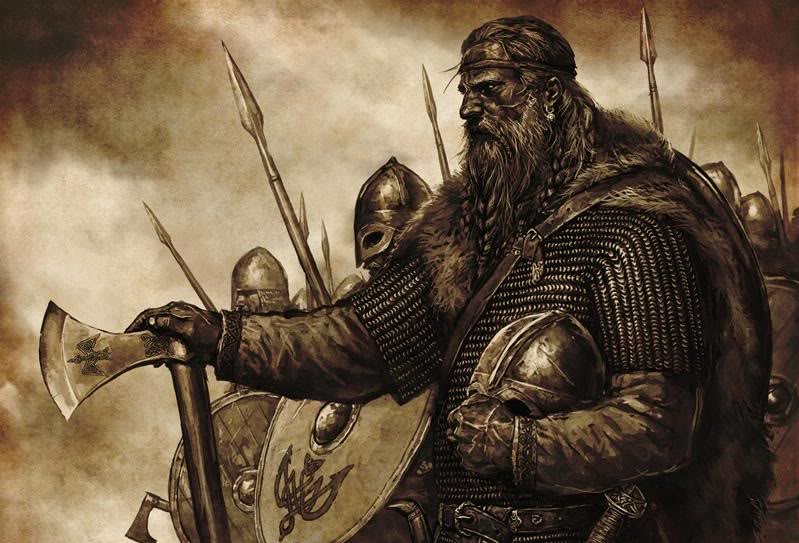
\includegraphics[width=\columnwidth]{viking1}
\end{figure}

\paragraph{Nosquam}

Naming Scheme: Latin, Any

\subsection{Ubris Furor}

Naming Scheme: Persian, Hebrew, Arabic, and Mongolian

% Between the lines of my journals is the struggle with Humankind's view of itself. The motives of our darkest past wells up and with which we must not only live but also contend. The land is haunted by the tragedies of its past made manifest in a parasitic curse that terrorises the land. 

%\paragraph{Nes} What you have here is a Viking themed Death World. The entire land is menaced by a terrible phantasmal parasite that infects any living organism. Over one third of the Kingdom is infected in a colossal biome known as the Phantasmal Forest. To survive, the people here have adapted to become some of the hardest motherfuckers to have ever lived, but at a great cost. Forget the advancement of culture, of science, and of common understanding. They are trapped in a dark age of perpetual war. The goal of every man, woman, and child, is to survive and keep the human race alive. 

\section{Culture}
Culture is an immensely important and often ignored most of most RPGs, and there is a tendency for most of them to be "generic medieval". I describe them as such because they tend not to actually capture the glory of the medieval period, its tragedies and culture of treachery. 

There is a great disparity in the cultural advancement of the provinces in Haeckel. Additionally, while a particular region could be of a certain culture level, it is entirely possible that the outskirts are more savage - as is especially the case with Brouliard where it has embraced the Renaissance in the cities but is still trapped in the Late Medieval Age in its vast farmlands. 

Thus I have created a Culture Level system that gives a general idea of the level of development. It also helps drive home to the players and GMs the impactful differences between the cultures - and so for this reason I see it as invaluable. 

\paragraph{CL 0 - Savage}

\paragraph{CL 1 - Stone Age}

\paragraph{CL 2 - Bronze Age}

\paragraph{CL 3 - Iron Age}

\paragraph{CL 4 - Classical}

\paragraph{CL 5 - Dark Age}

\paragraph{CL 6 - Early Medieval} 

\paragraph{CL 7 - Medieval}

\paragraph{CL 8 - Chivalric}

\paragraph{CL 9 - Renaissance}

Avalonia is completely crippled and is literally in the stone age. Nes is perpetually trapped in the dark age due to its own troubles. One of the aims of Haeckel was to provide rich cultures that have impact on the players. 

There is no "generic medieval" here. The Medieval realm of Midgaard really drives home what Medieval means, in every sense, good and bad. North Wall is the howling abyss of the setting, a region of immeasurable vastness, it is in literal terms the land of adventure.

\section{Technology Overview} 
% Despite not having advanced cartographical skills, the setting is actually quite advanced. The cannon is a technology in widespread use. Gunpowder is prevalent in some areas, though not mass produceable yet. Dark whispers suggest that Ablon is secretly developing the steam engine.
Firstly, it is important to recognize that Haeckel's purpose is not to recreate historical time periods. We draw from history to promote verisimilitude. Haeckel has developed technologically in a different way from Earth. Culturally, brouliard has reached the Enlightenment and technologically Ablon has advanced beyond that. However, the Age of Colonialism never occurred. The advanced mathematical skills needed to develop cartography has not occurred yet. Thus maps have a tendency to be misleading, or worse, horribly inaccurate. 

\subsection{Cartography}

\subsection{Gunpowder} Gunpowder has been around for awhile and is primarily used with siege weaponry. Some of the more advanced nations have developed flintlock pistols but they are not in common use within their militaries. During the civil war Necromancy was used in warfare and inevitably a large zombie army was summoned. Small arm gunpowder weaponry proved useless against them – and phalanxes were not so effective either. This has meant that there has not been a large scale shift towards using such weaponry – however their use in warfare against armour is recognized. The circumstances of the different provinces has led to different strategies in warfare being preferred.

\subsection{Communication}

\subsection{Travel}

\subsection{Printing Press}

\subsection{Education} 

In the world of Haeckel, each nation is actively seeking to steal the technological secrets of the others. Gunpowder and siege weaponry are some of the easiest and fastest to steal - and hence even some of the most barbaric lands have access to cannons (though not necessarily many of them due to poor economies). 

% La_Rochelle_by_Radojavor
\begin{figure}[h]
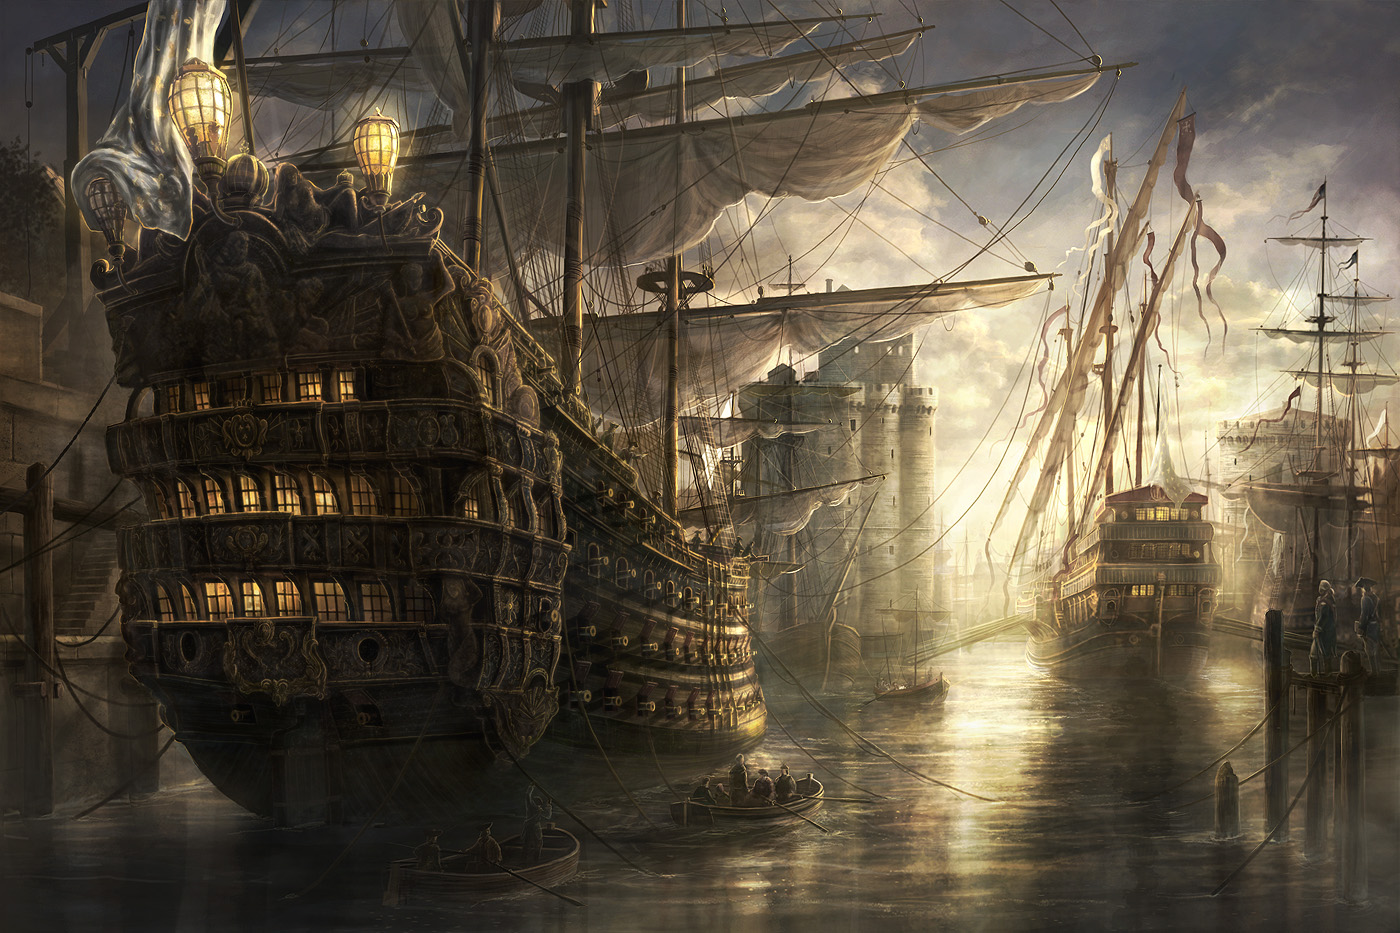
\includegraphics[width=\columnwidth]{La_Rochelle_by_Radojavor}
\end{figure}

\section{Lexicon} 

\section{Adventure Sites}

\end{multicols}